\section{Thực nghiệm mining và kiểm chứng dữ liệu xuất}
\label{sec:mining-exp}
Thực nghiệm mở rộng dùng revision \code{c4388f1}. Từ thứ tự 500 ID đã cố định trong manifest, 300 ảnh đầu làm tập tuyển chọn/train, 100 ảnh tiếp theo làm validation và 100 ảnh cuối làm test. Đây là phép chia phục vụ nghiên cứu nhỏ trên COCO val2017, không phải tập train/test chính thức của COCO. Các số AP của ba checkpoint ở phần trước vẫn được tính trên đủ 500 ảnh với checkpoint chưa fine-tune; các checkpoint fine-tune không được đánh giá lại trên những ảnh đã dùng train để báo kết quả tổng quát hóa.

Mining chỉ truy cập tập train. Annotation crowd bị loại khỏi bộ YOLO của thí nghiệm; box được chặn trong biên ảnh và chỉ giữ diện tích dương. Tập tuyển chọn có 300 ảnh và 2.099 box. Ba tập được tách bằng ID ảnh; nghiên cứu chưa bổ sung loại trùng ngữ nghĩa hoặc nhóm ảnh gần giống giữa các split. Không sử dụng nhãn tự động.

Random, Weighted, Diversity và Rare-first có ngân sách 150 ảnh. Diversity dùng 150 cụm và chọn một đại diện mỗi cụm; seed chọn bằng 42. Quality dùng ngưỡng 0,5; Boxes yêu cầu ít nhất hai box; Class yêu cầu có lớp person; Quota và Coverage đặt quota ba ảnh/lớp với giới hạn 150; Balance dùng median theo số ảnh chứa lớp. Các bộ lọc và quota có thể trả ít hơn giới hạn nên không được xem là đối chứng cùng ngân sách cho mọi hàng.

Thời gian chọn lấy trung vị ba lần sau một lượt warm-up trên collection đã nạp, chạy CPU. Weighted và Diversity bao gồm tính điểm hoặc trích đặc trưng/phân cụm trong mỗi lần đo; không dùng báo cáo tính sẵn để che chi phí chuẩn bị. Thời gian không gồm export. Hàng full chỉ tham chiếu collection đầu vào nên thời gian gần bằng không, không phải chi phí đọc dữ liệu từ đĩa.

\begin{table}[H]\centering\small
\caption{Benchmark tuyển chọn trên 300 ảnh; IR chỉ tính các lớp hiện diện}
\begin{tabular}{lrrrrr}
\toprule
Cách chọn & Ảnh & Box & Lớp & IR & Chọn (ms) \\
\midrule
full & 300 & 2099 & 77 & 167.0 & 0.0 \\
random & 150 & 1070 & 76 & 79.0 & 9.3 \\
weighted & 150 & 1410 & 77 & 69.0 & 4693.7 \\
diversity & 150 & 1172 & 75 & 87.0 & 5980.4 \\
rare-first & 150 & 904 & 76 & 42.0 & 4337.5 \\
coverage & 97 & 835 & 77 & 45.0 & 130.2 \\
quota & 97 & 835 & 77 & 45.0 & 93.7 \\
quality & 150 & 1160 & 74 & 91.0 & 4374.7 \\
boxes & 150 & 1266 & 74 & 92.0 & 10.0 \\
class & 150 & 1321 & 69 & 150.0 & 9.2 \\
balance & 212 & 1553 & 77 & 111.0 & 141.0 \\
\bottomrule
\end{tabular}

\end{table}
Quota và Coverage tạo cùng tập ảnh do đi qua cùng hàm greedy; chênh lệch thời gian đo không phải bằng chứng khác biệt thuật toán. Balance có thể giữ hơn 150 ảnh và không bị áp cùng ngân sách. Weighted giữ nhiều box hơn Random dù số ảnh bằng nhau, nên thực nghiệm huấn luyện cùng số ảnh chưa phải cùng số đối tượng được quan sát. Khi đánh giá hiệu quả chọn cần công bố cả hai đơn vị.

\begin{figure}[H]\centering
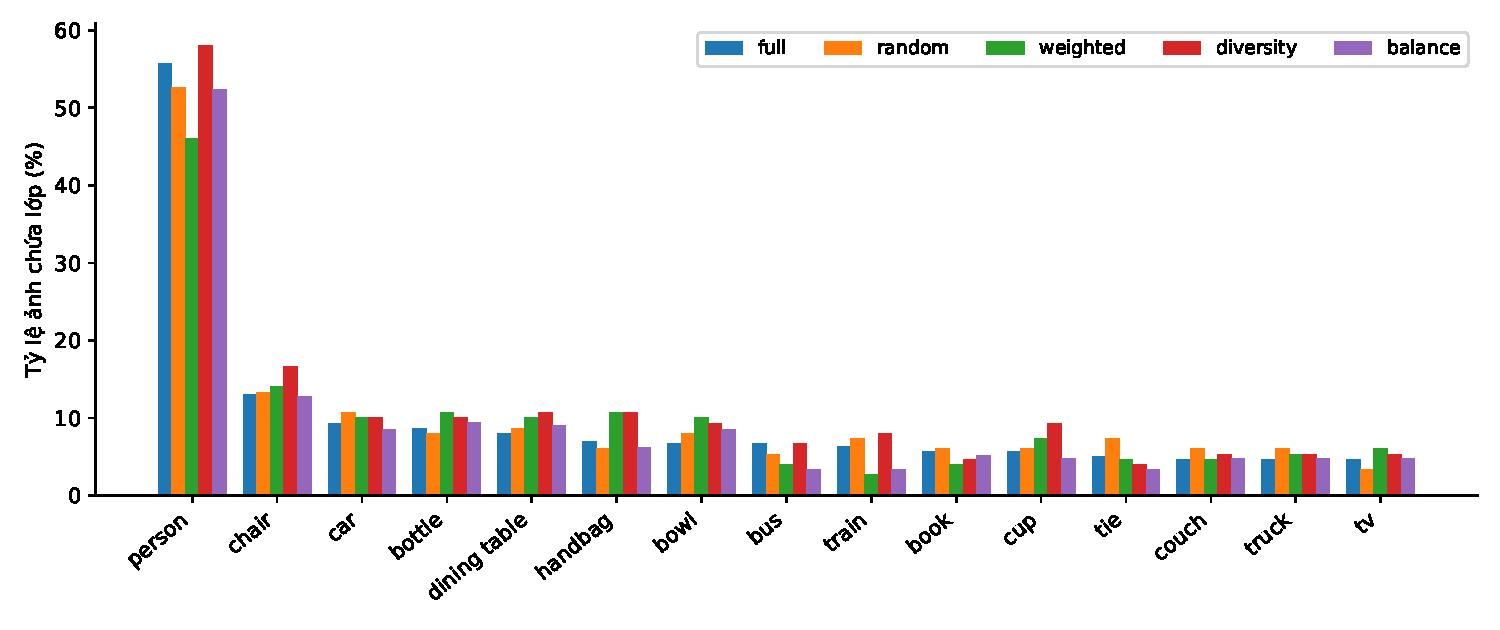
\includegraphics[width=\textwidth]{klygo/mining_distribution.pdf}
\caption{Phân bố 15 lớp phổ biến nhất của tập đầu vào, chuẩn hóa theo số ảnh của từng tập}
\end{figure}
\begin{figure}[H]\centering
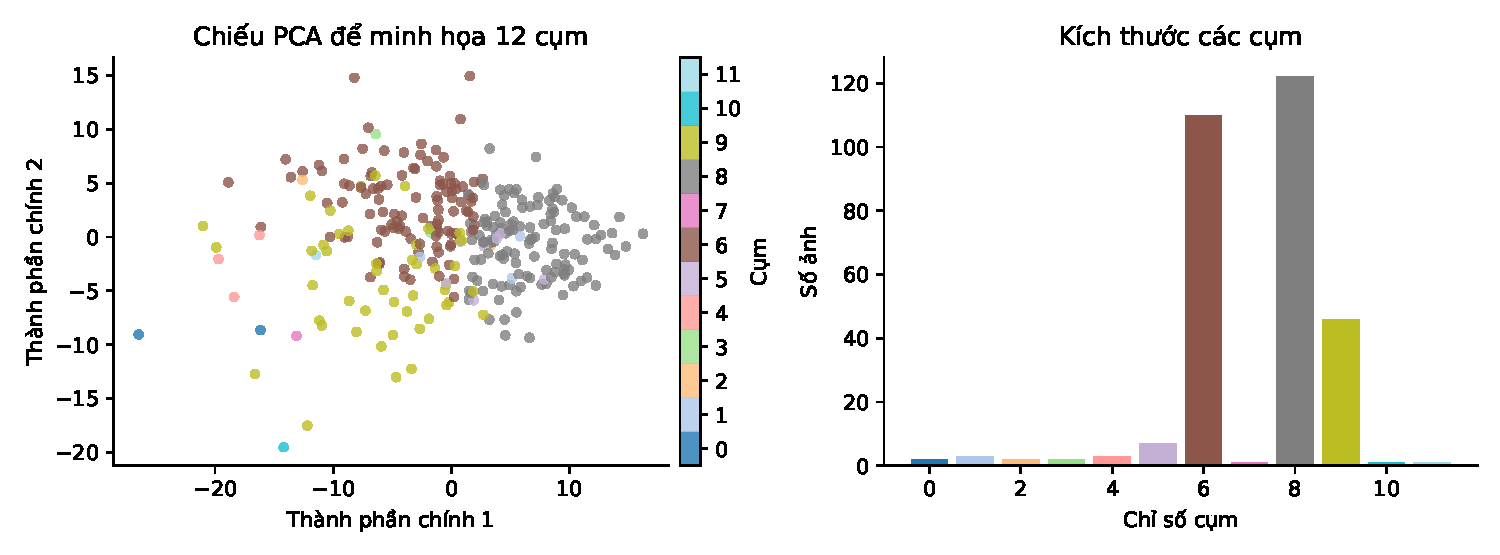
\includegraphics[width=\textwidth]{klygo/mining_clusters.pdf}
\caption{Minh họa 12 cụm trên 300 ảnh; PCA chỉ dùng để vẽ, không dùng để chọn mẫu}
\end{figure}
Hình phân cụm dùng $K=12$ để quan sát và được lưu riêng với cấu hình tuyển chọn $K=150$. Phân tích thành phần chính (PCA) chiếu dữ liệu lên hai hướng có phương sai lớn để minh họa. Khoảng cách trên mặt phẳng này không bảo toàn toàn bộ khoảng cách 726 chiều; ảnh gần nhau trên hình chưa đủ để kết luận là ảnh trùng. Không lựa chọn $K$ hay trọng số dựa trên điểm test.

\subsection{Từ export annotation đến bộ dữ liệu huấn luyện}
Trong revision này, \code{Detections.export(format="yolo")} ghi nhãn, registry lớp và manifest, không sao chép ảnh nguồn. Script thực nghiệm ghép ảnh theo \code{source\_path}, đổi tên tương ứng \code{label\_file}, rồi tạo YAML với đường dẫn train/val/test. Việc ghép ảnh và tạo YAML là bước chuẩn bị bổ sung của thực nghiệm, không được quy cho API export tự thực hiện.

Mỗi phương pháp được kiểm tra số ID duy nhất, tập ID là tập con của train, số ảnh/box và số box theo từng lớp sau khi đọc lại bằng \code{datasets.load}. Các kiểm tra đều đạt; nội dung đầu vào được đối chiếu trước và sau mining để xác nhận không bị thay đổi. Kiểm tra round-trip này xác nhận tính toàn vẹn cấu trúc và số nhãn, không thay thế đánh giá chất lượng annotation.

Export đánh lại class ID liên tục theo registry hiện diện của từng tập. Vì các tập có thể thiếu những lớp khác nhau, bộ nhãn được ánh xạ lại theo tên về cùng thứ tự 80 lớp COCO trước khi train. Script \code{prepare\_training\_canonical.py} kiểm tra bảo toàn số box theo tên lớp sau phép đổi ID. Lượt thử trước khi phát hiện khác biệt registry đã được dừng và giữ riêng; chỉ kết quả trong \code{training\_canonical} được dùng ở bảng và biểu đồ huấn luyện.

\section{Fine-tune trên dữ liệu được tuyển chọn}
\label{sec:mining-train}
Bốn cấu hình train là Full (300 ảnh), Random, Weighted và Diversity (mỗi tập 150 ảnh). Mọi lượt bắt đầu từ cùng checkpoint YOLOv8n COCO pretrained. Mỗi cấu hình chạy năm epoch với ba seed huấn luyện 42, 43 và 44; tập được chọn giữ nguyên seed 42. Độ lệch chuẩn vì vậy mô tả biến thiên huấn luyện có điều kiện trên các tập đã cố định, chưa bao gồm biến thiên khi chọn lại dữ liệu.

Vocabulary của model và YAML được giữ đủ 80 lớp để đầu ra có ý nghĩa nhất quán và sử dụng nguyên checkpoint khởi tạo. Tập full train có 77 lớp hiện diện; số lớp có ground truth trong test là 73. Các lớp ít mẫu khiến AP nhạy với một vài dự đoán; không diễn giải trung bình trên tập test nhỏ như mức chất lượng của toàn bộ COCO.

Thiết lập gồm kích thước 320, batch tám, FP32, AdamW, learning rate đầu 0,001, hệ số cuối 0,1, không warm-up, không mosaic/mixup và không early stopping. Số worker đọc dữ liệu bằng không. Sử dụng checkpoint epoch cuối, không chọn checkpoint theo tập test. Chất lượng được đo bằng metric bbox của Ultralytics trên 100 ảnh test, confidence 0,001, NMS IoU 0,7, max detections 100. Quy trình huấn luyện và tham số được lưu kèm \citep{ultralyticsTrain}; phiên bản thực thi được khóa ở 8.3.228. AP ở mục này không trộn với kết quả COCOeval 500 ảnh/kích thước 640 ở phần trước.

\begin{table}[H]\centering\small
\caption{Fine-tune năm epoch: trung bình và độ lệch chuẩn mẫu qua ba seed}
\begin{tabular}{lrrrr}
\toprule
Tập train & Ảnh & AP (\%) & AP50 (\%) & Train (s) \\
\midrule
full & 300 & 10.38 $\pm$ 1.91 & 17.28 & 52.4 \\
random & 150 & 10.10 $\pm$ 0.61 & 16.20 & 30.4 \\
weighted & 150 & 10.38 $\pm$ 0.55 & 16.83 & 30.7 \\
diversity & 150 & 8.00 $\pm$ 1.85 & 14.14 & 30.6 \\
\bottomrule
\end{tabular}

\end{table}
\begin{figure}[H]\centering
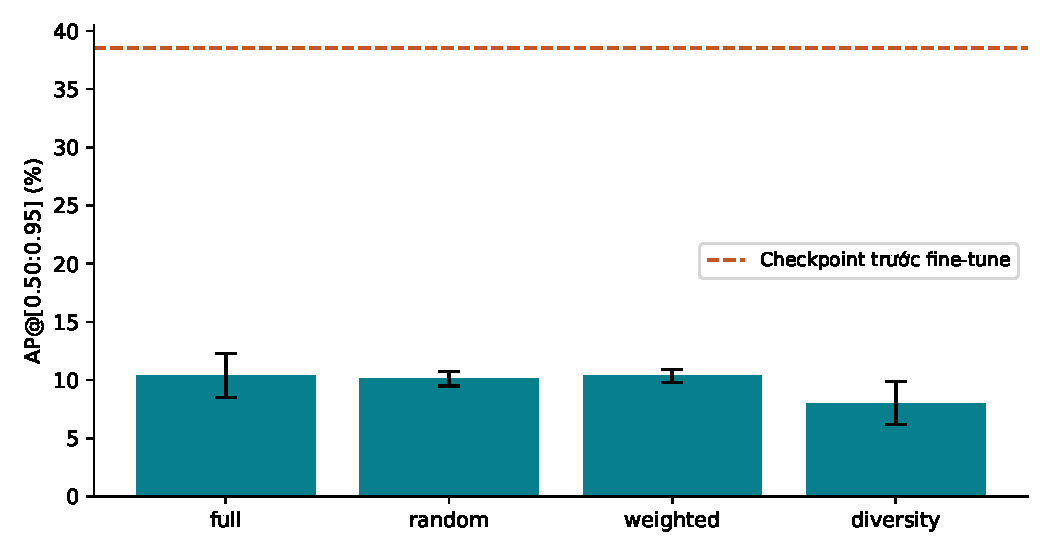
\includegraphics[width=.88\textwidth]{klygo/mining_training.pdf}
\caption{Chất lượng sau fine-tune và checkpoint ban đầu trên cùng tập test}
\end{figure}
Checkpoint ban đầu đạt AP 38.52\% trên cùng 100 ảnh test ở kích thước 320. Weighted chênh +0.28 điểm phần trăm AP so với Random cùng 150 ảnh. Diversity chênh -2.10 điểm phần trăm AP so với Random cùng 150 ảnh. Các chênh lệch là mô tả mẫu; ba seed không đủ để khẳng định khác biệt có ý nghĩa thống kê hoặc ưu thế trên các tập dữ liệu khác. Độ lệch chuẩn phản ánh biến thiên huấn luyện, không phải khoảng tin cậy do lấy mẫu ảnh test.

Thời gian train là thời gian tường của lời gọi train, gồm khởi tạo trainer, lưu checkpoint và xử lý validation bên trong thư viện, không gồm đánh giá test riêng. Đây là so sánh cùng epoch: full có khoảng gấp đôi số batch cập nhật so với mỗi tập con. Chi phí mining cũng cần cộng vào khi xét tổng thời gian. Năm epoch và 100 ảnh test là một thực nghiệm thăm dò; không đủ để xếp hạng phương pháp trên toàn COCO hay suy ra kết quả học từ đầu. Fine-tune ngắn có thể giảm AP so với checkpoint ban đầu do tập nhỏ và thay đổi phân bố; kết quả giảm vẫn được báo cáo.

\section{Benchmark framework gốc và các chế độ Klygo}
\label{sec:execution-exp}
Thực nghiệm dùng YOLOv8n và YOLO-World v2 small ở revision \code{c4388f1}, theo sáu cấu hình đã phân biệt ở Hình~\ref{fig:execution-paths} và bảng tương ứng trong chương thiết kế. Cả sáu nhánh được đo lại trong phiên ngày 07/11/2026; không ghép một hàng mới vào kết quả năm nhánh của phiên trước. Mỗi cặp model/chế độ được nạp trong tiến trình riêng. Đầu vào là cùng 100 ảnh JPEG theo thứ tự manifest, đặt tên để thứ tự duyệt thư mục được xác định. Mỗi nhánh có một lượt warm-up toàn tập rồi ba lượt đo toàn tập; batch một, FP32, kích thước 640, confidence 0,25, IoU 0,7 và max detections 100. Không thay vocabulary YOLO-World.

Lượt thăm dò ở confidence 0,001 dừng tại Klygo native do backend trả box có chiều rộng hoặc chiều cao bằng không, bị validator từ chối. Log và các kết quả Raw của lượt này được giữ riêng, không ghép vào bảng. Benchmark đầy đủ được chạy lại ở confidence 0,25 cho tất cả các nhánh, không loại ảnh gây lỗi. Đây là cấu hình phục vụ suy luận thông thường; chưa chứng minh revision mới hoạt động với mọi box ở ngưỡng rất thấp. Không dùng bảng thời gian này làm thời gian tính AP ở confidence 0,001.

Timer bao gồm giải mã nguồn, suy luận, hậu xử lý và trả kết quả công khai; không gồm nạp trọng số. Với stream, timer kéo dài đến khi tiêu thụ hết iterator. Thời điểm kết quả đầu tiên được quan sát từ phía người gọi, nên ở non-stream/native nó bao gồm chờ hoàn thành collection; không được gọi là độ trễ suy luận của một frame. CUDA được đồng bộ tại ranh giới đo và khi nhận kết quả đầu. Việc chuẩn hóa dự đoán để đối chiếu được thực hiện trong một lượt riêng, ngoài timer.

RAM là RSS đỉnh được lấy mẫu mỗi 10 ms trong tiến trình; VRAM là đỉnh bộ nhớ tensor do PyTorch cấp phát, không phải toàn bộ bộ nhớ thiết bị do trình điều khiển báo. Các cột bộ nhớ là MiB tuyệt đối và có bao gồm model/runtime. Số liệu là trung vị ba lượt. Chênh lệch bộ nhớ so với trước mỗi lượt cũng được lưu trong JSON; phép đo ngắn chưa kiểm chứng giới hạn bộ nhớ của một video kéo dài.

\begin{table}[H]\centering\small
\caption{YOLOv8n: cùng 100 ảnh, các chế độ thực thi}
\begin{tabular}{lrrrrr}
\toprule
Chế độ & Giây & Ảnh/s & Đầu (ms) & RAM & VRAM \\
\midrule
raw & 1.93 & 51.91 & 1926.5 & 1164 & 46 \\
raw stream & 2.14 & 46.77 & 23.7 & 1075 & 46 \\
native & 2.24 & 44.74 & 2235.0 & 1137 & 46 \\
native backend stream & 1.99 & 50.23 & 1990.8 & 1071 & 46 \\
managed & 1.83 & 54.70 & 1828.2 & 1062 & 38 \\
managed stream & 1.99 & 50.26 & 35.1 & 1060 & 38 \\
\bottomrule
\end{tabular}

\end{table}
\begin{table}[H]\centering\small
\caption{YOLO-World: cùng 100 ảnh, các chế độ thực thi}
\begin{tabular}{lrrrrr}
\toprule
Chế độ & Giây & Ảnh/s & Đầu (ms) & RAM & VRAM \\
\midrule
raw & 2.84 & 35.25 & 2836.5 & 1253 & 137 \\
raw stream & 2.60 & 38.47 & 27.2 & 1171 & 137 \\
native & 3.25 & 30.77 & 3250.2 & 1201 & 137 \\
native backend stream & 2.99 & 33.40 & 2994.0 & 1121 & 137 \\
managed & 2.52 & 39.71 & 2518.2 & 1125 & 128 \\
managed stream & 2.54 & 39.33 & 41.9 & 1126 & 128 \\
\bottomrule
\end{tabular}

\end{table}
\begin{figure}[H]\centering
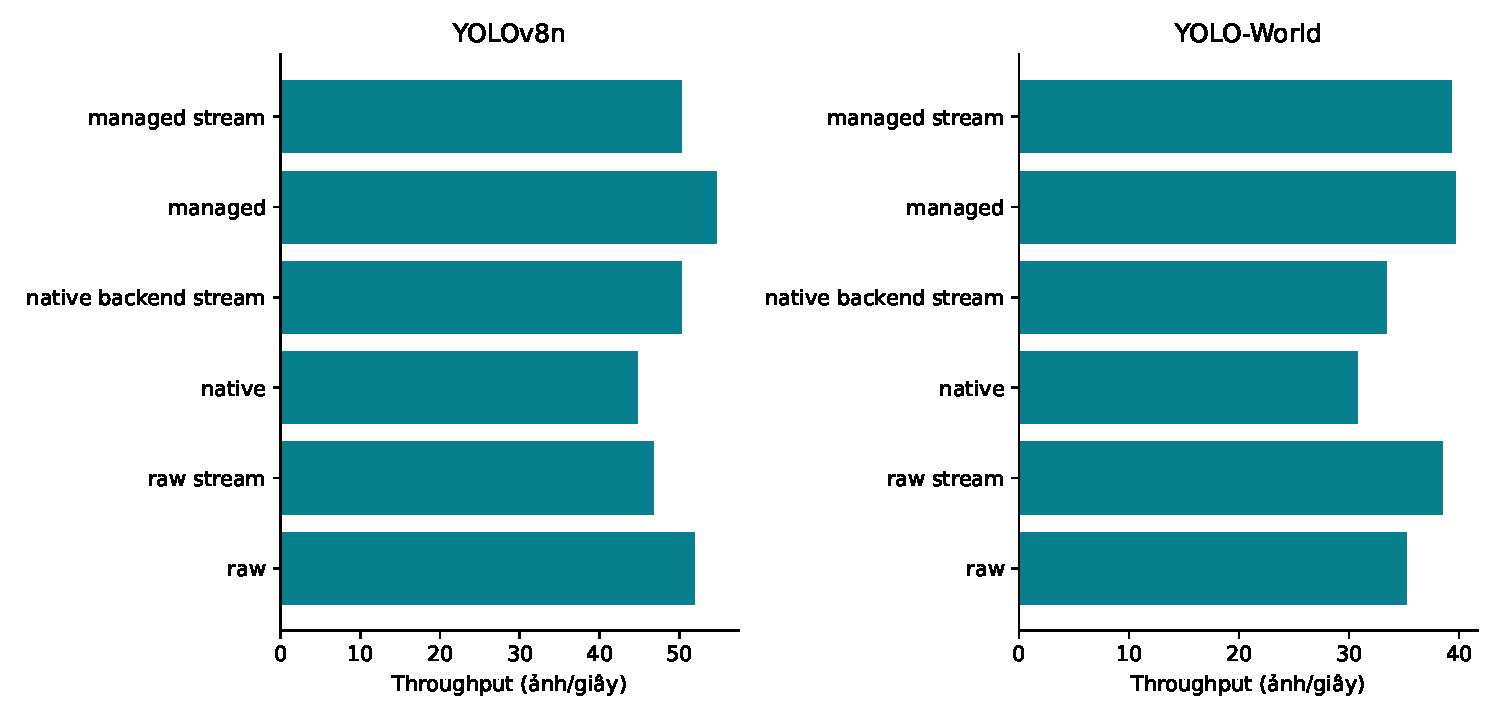
\includegraphics[width=\textwidth]{klygo/execution_throughput.pdf}
\caption{Throughput của framework gốc và các đường thực thi Klygo}
\end{figure}
YOLOv8n: chênh lệch thời gian toàn tập so với Raw là native +16.0\%, native backend stream +3.3\%, managed -5.1\%, managed stream +3.3\%. Dấu dương biểu thị chậm hơn, dấu âm biểu thị nhanh hơn trong phép đo này.

Đối chiếu YOLOv8n có 0/500 cặp frame vượt tiêu chí tương đương: cùng số box, class và sai số tọa độ không quá 0,01 pixel, score không quá 0,001. Sai số lớn nhất theo cách ghép class/score là 0.000000 pixel và 0.000000 điểm score. Phép kiểm tra này dùng dự đoán framework làm tham chiếu, không gọi đó là ground truth.

YOLO-World: chênh lệch thời gian toàn tập so với Raw là native +14.6\%, native backend stream +5.5\%, managed -11.2\%, managed stream -10.4\%. Dấu dương biểu thị chậm hơn, dấu âm biểu thị nhanh hơn trong phép đo này.

Đối chiếu YOLO-World có 0/500 cặp frame vượt tiêu chí tương đương: cùng số box, class và sai số tọa độ không quá 0,01 pixel, score không quá 0,001. Sai số lớn nhất theo cách ghép class/score là 0.000000 pixel và 0.000000 điểm score. Phép kiểm tra này dùng dự đoán framework làm tham chiếu, không gọi đó là ground truth.

Raw trả kiểu dữ liệu của framework, còn Klygo bổ sung container, identity và metadata. Vì đầu ra có chức năng khác nhau, chênh lệch Raw--Klygo là chi phí hoặc lợi ích của đường xử lý hoàn chỉnh, không cô lập thời gian kernel mạng. Native--Managed giúp quan sát thêm ảnh hưởng điều phối nguồn. Không dùng phép đo này để tuyên bố kiến trúc mạng đã được tối ưu, hoặc mọi cấu hình stream đều nhanh hơn non-stream.

Các chế độ được chạy nối tiếp trong những tiến trình khác nhau, chưa hoán đổi thứ tự theo một thiết kế ngẫu nhiên cân bằng. Tải hệ điều hành, cache đĩa và trạng thái nhiệt/xung GPU vẫn có thể tạo nhiễu; ba lượt đo không loại bỏ được các yếu tố đó. Những chênh lệch nhỏ cần được kiểm tra lại trên nhiều phiên đo trước khi xem là cải thiện hiệu suất ổn định.

\section{Ảnh hưởng của worker và prefetch}
\label{sec:scheduling-exp}
Thực nghiệm tiếp theo giữ chế độ Managed stream và cùng toàn bộ cấu hình model, dữ liệu, phần cứng, ngưỡng, warm-up cùng số lượt đo của benchmark sáu mode. Chỉ thay cặp (workers, prefetch), ký hiệu (W,P). Mỗi cấu hình được nạp ở một tiến trình riêng; tham chiếu (1,1) lấy từ Managed stream của cùng phiên đo sáu mode. Không chạy huấn luyện hoặc một benchmark GPU khác đồng thời.

Các cặp được cố định trước khi chạy: (0,0), (1,1), (2,1), (4,1), (2,2), (2,4). Nhánh (0,0) là chuẩn bị tuần tự. Nhóm (1,1), (2,1), (4,1) giữ P=1 để khảo sát số worker; nhóm (2,1), (2,2), (2,4) giữ W=2 để khảo sát độ sâu hàng đợi. Batch vẫn bằng một, nên kết quả chưa đại diện cho khả năng giải mã nhiều ảnh trong cùng một batch lớn.

\begin{table}[H]\centering\small
\caption{YOLOv8n Managed stream: ảnh hưởng của worker/prefetch trên 100 ảnh}
\begin{tabular}{rrrrrrr}
\toprule
W & P & Giây & Min--max (s) & Ảnh/s & Đầu (ms) & RAM \\
\midrule
0 & 0 & 2.05 & 2.01--2.17 & 48.84 & 32.6 & 1060 \\
1 & 1 & 1.99 & 1.86--2.06 & 50.26 & 35.1 & 1060 \\
2 & 1 & 1.98 & 1.88--2.05 & 50.57 & 38.9 & 1063 \\
4 & 1 & 2.17 & 2.08--2.23 & 46.03 & 33.9 & 1073 \\
2 & 2 & 1.83 & 1.83--1.95 & 54.67 & 37.8 & 1063 \\
2 & 4 & 1.82 & 1.81--1.89 & 55.05 & 39.3 & 1063 \\
\bottomrule
\end{tabular}

\end{table}
\begin{table}[H]\centering\small
\caption{YOLO-World Managed stream: ảnh hưởng của worker/prefetch trên 100 ảnh}
\begin{tabular}{rrrrrrr}
\toprule
W & P & Giây & Min--max (s) & Ảnh/s & Đầu (ms) & RAM \\
\midrule
0 & 0 & 2.80 & 2.75--2.87 & 35.76 & 40.8 & 1123 \\
1 & 1 & 2.54 & 2.52--2.57 & 39.33 & 41.9 & 1126 \\
2 & 1 & 2.53 & 2.51--2.55 & 39.55 & 42.0 & 1139 \\
4 & 1 & 2.56 & 2.54--2.74 & 39.03 & 41.2 & 1128 \\
2 & 2 & 2.57 & 2.53--2.61 & 38.93 & 45.9 & 1127 \\
2 & 4 & 2.55 & 2.55--2.56 & 39.27 & 42.3 & 1126 \\
\bottomrule
\end{tabular}

\end{table}
Các cột thời gian toàn tập, throughput, thời gian tới kết quả đầu và RSS đỉnh là trung vị ba lượt; cột min--max là khoảng quan sát của thời gian toàn tập qua ba lượt, không phải khoảng tin cậy. RAM dùng MiB, lấy mẫu 10 ms như phần trước. Các file JSON còn lưu đỉnh VRAM và chênh lệch bộ nhớ so với trước mỗi lượt. RSS phụ thuộc cả model/runtime và allocator, nên không diễn giải mọi chênh lệch RSS thành dung lượng riêng của hàng đợi prefetch.

\begin{figure}[H]\centering
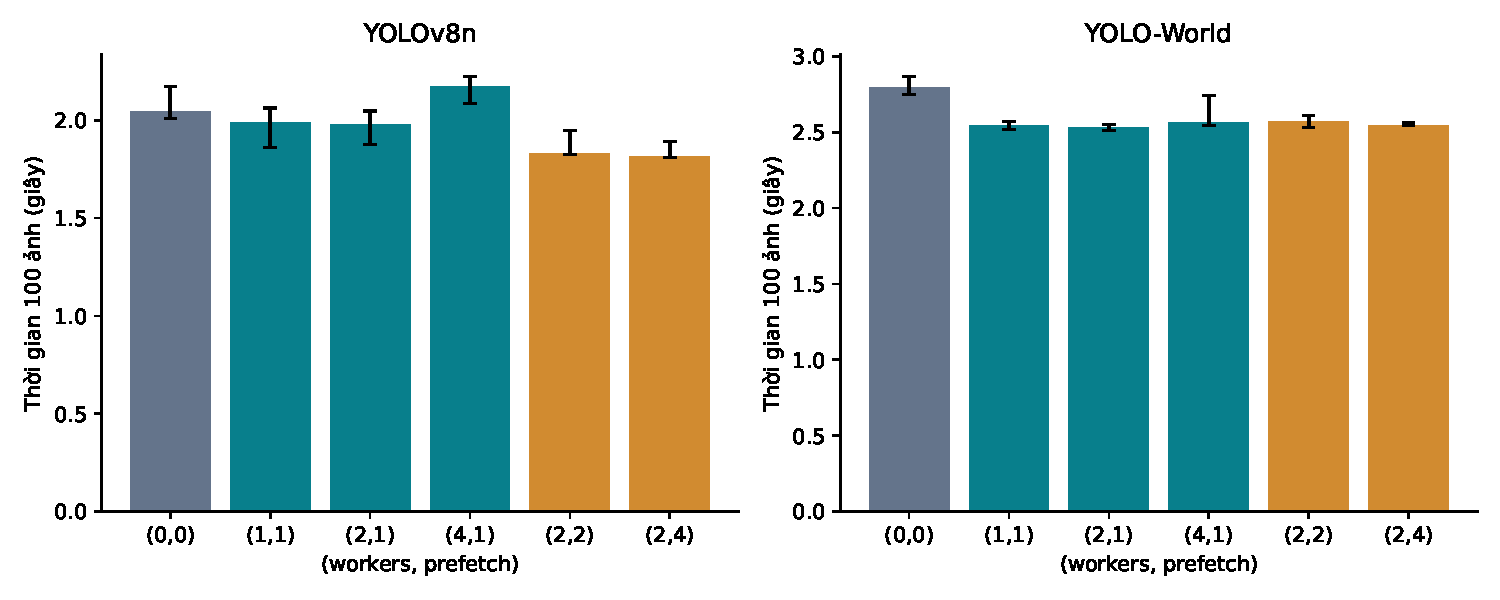
\includegraphics[width=\textwidth]{klygo/scheduling_comparison.pdf}
\caption{Thời gian xử lý theo cặp worker/prefetch; cột là trung vị, thanh sai số biểu diễn min--max của ba lượt}
\end{figure}
YOLOv8n: trung vị nhỏ nhất trong các cấu hình đã đo là (2,4) với 1.82 s; mặc định (1,1) là 1.99 s và tuần tự (0,0) là 2.05 s. Đây là mô tả phiên đo, không khẳng định cấu hình tối ưu trên mọi workload.

Sáu cấu hình YOLOv8n có 0/600 cặp frame vượt tiêu chí tương đương so với Raw, với cùng ngưỡng sai số như benchmark sáu mode.

YOLO-World: trung vị nhỏ nhất trong các cấu hình đã đo là (2,1) với 2.53 s; mặc định (1,1) là 2.54 s và tuần tự (0,0) là 2.80 s. Đây là mô tả phiên đo, không khẳng định cấu hình tối ưu trên mọi workload.

Sáu cấu hình YOLO-World có 0/600 cặp frame vượt tiêu chí tương đương so với Raw, với cùng ngưỡng sai số như benchmark sáu mode.

Chọn cấu hình sử dụng còn phụ thuộc độ trễ chấp nhận được và ngân sách RAM. Tăng worker/prefetch không có cam kết giảm thời gian đơn điệu; lợi ích chỉ xuất hiện khi nó giúp giải mã theo kịp mô hình, trong khi các chi phí đồng bộ và giữ pixel vẫn tồn tại. Phiên đo hữu hạn này chưa đánh giá nguồn video dài, batch lớn hay đọc dữ liệu qua mạng. Vì các cấu hình chưa được chạy theo thứ tự ngẫu nhiên cân bằng, kết quả cần được tái kiểm chứng trước khi dùng làm khuyến nghị triển khai chung.
